\section{eo\-Stochastic\-Universal\-Select$<$ EOT $>$ Class Template Reference}
\label{classeo_stochastic_universal_select}\index{eoStochasticUniversalSelect@{eoStochasticUniversalSelect}}
eo\-Stochastic\-Universal\-Select: select an individual proportional to her stored fitness value, but in contrast with eo\-Stochastic\-Universal\-Select, get rid of most finite sampling effects by doing all selections in one go, using a single random number.  


{\tt \#include $<$eo\-Stochastic\-Universal\-Select.h$>$}

Inheritance diagram for eo\-Stochastic\-Universal\-Select$<$ EOT $>$::\begin{figure}[H]
\begin{center}
\leavevmode
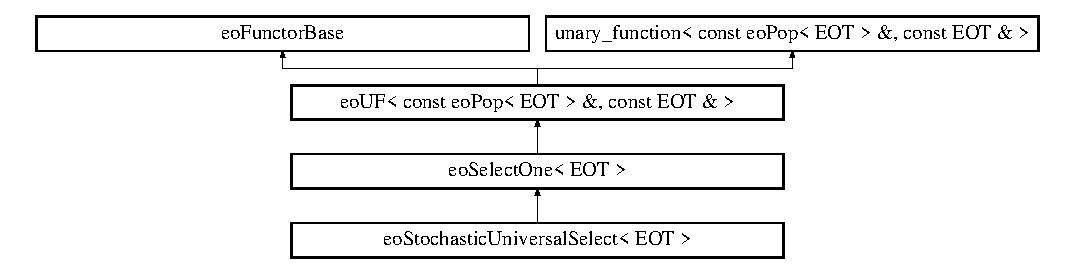
\includegraphics[height=3.23699cm]{classeo_stochastic_universal_select}
\end{center}
\end{figure}
\subsection*{Public Member Functions}
\begin{CompactItemize}
\item 
{\bf eo\-Stochastic\-Universal\-Select} (const {\bf eo\-Pop}$<$ {\bf EOT} $>$ \&pop={\bf eo\-Pop}$<$ {\bf EOT} $>$())\label{classeo_stochastic_universal_select_a0}

\begin{CompactList}\small\item\em Sanity check. \item\end{CompactList}\item 
void {\bf setup} (const {\bf eo\-Pop}$<$ {\bf EOT} $>$ \&\_\-pop)\label{classeo_stochastic_universal_select_a1}

\begin{CompactList}\small\item\em virtual function to setup some population stats (for instance eo\-Proportional can benefit greatly from this) \item\end{CompactList}\item 
const {\bf EOT} \& {\bf operator()} (const {\bf eo\-Pop}$<$ {\bf EOT} $>$ \&\_\-pop)\label{classeo_stochastic_universal_select_a2}

\begin{CompactList}\small\item\em do the selection, \item\end{CompactList}\end{CompactItemize}
\subsection*{Private Types}
\begin{CompactItemize}
\item 
typedef std::vector$<$ unsigned $>$ {\bf Index\-Vec}\label{classeo_stochastic_universal_select_y0}

\end{CompactItemize}
\subsection*{Private Attributes}
\begin{CompactItemize}
\item 
Index\-Vec {\bf indices}\label{classeo_stochastic_universal_select_r0}

\end{CompactItemize}


\subsection{Detailed Description}
\subsubsection*{template$<$class EOT$>$ class eo\-Stochastic\-Universal\-Select$<$ EOT $>$}

eo\-Stochastic\-Universal\-Select: select an individual proportional to her stored fitness value, but in contrast with eo\-Stochastic\-Universal\-Select, get rid of most finite sampling effects by doing all selections in one go, using a single random number. 



Definition at line 44 of file eo\-Stochastic\-Universal\-Select.h.

The documentation for this class was generated from the following file:\begin{CompactItemize}
\item 
eo\-Stochastic\-Universal\-Select.h\end{CompactItemize}
